\documentclass[dvipdfmx]{jarticle}
\usepackage{graphicx}
\usepackage[top=30truemm,bottom=30truemm,left=25truemm,right=25truemm]{geometry}
\usepackage{listings,jvlisting}

\lstset{
  basicstyle={\ttfamily},
  identifierstyle={\small},
  commentstyle={\smallitshape},
  keywordstyle={\small\bfseries},
  ndkeywordstyle={\small},
  stringstyle={\small\ttfamily},
  frame={tb},
  breaklines=true,
  columns=[l]{fullflexible},
  numbers=left,
  xrightmargin=0zw,
  xleftmargin=3zw,
  numberstyle={\scriptsize},
  stepnumber=1,
  numbersep=1zw,
  lineskip=-0.5ex
}

\begin{document}
\begin{titlepage}
    \begin{center}
        {\huge 情報科学実験A レポート4}
        \vspace{180pt}\\
        \begin{tabular}{rl}
            氏名 & 山久保孝亮\\
            所属 & 大阪大学基礎工学部情報科学科ソフトウェア科学コース\\
            学籍番号 & 09B22084\\
            提出日 & \today\\
            担当教員 & 繁田 浩功/桝井 晃基
        \end{tabular}
    \end{center}
\end{titlepage}
\section{実験ペアの名前および学籍番号}
\begin{table}[h]
    \centering
    \begin{tabular}{|c|c|}
        \hline
        学籍番号 & 名前\\\hline\hline
        09B22083 & 安川雄輝\\\hline
    \end{tabular}
    \caption{ペアの学籍番号と名前}
\end{table}
\section{送受信回路のステート・マシンの概要図}
送受信回路のステート・マシンの概要図は以下の図1,図2のようになった.
\begin{figure}[h]
    \begin{minipage}[b]{0.45\linewidth}
      \centering
      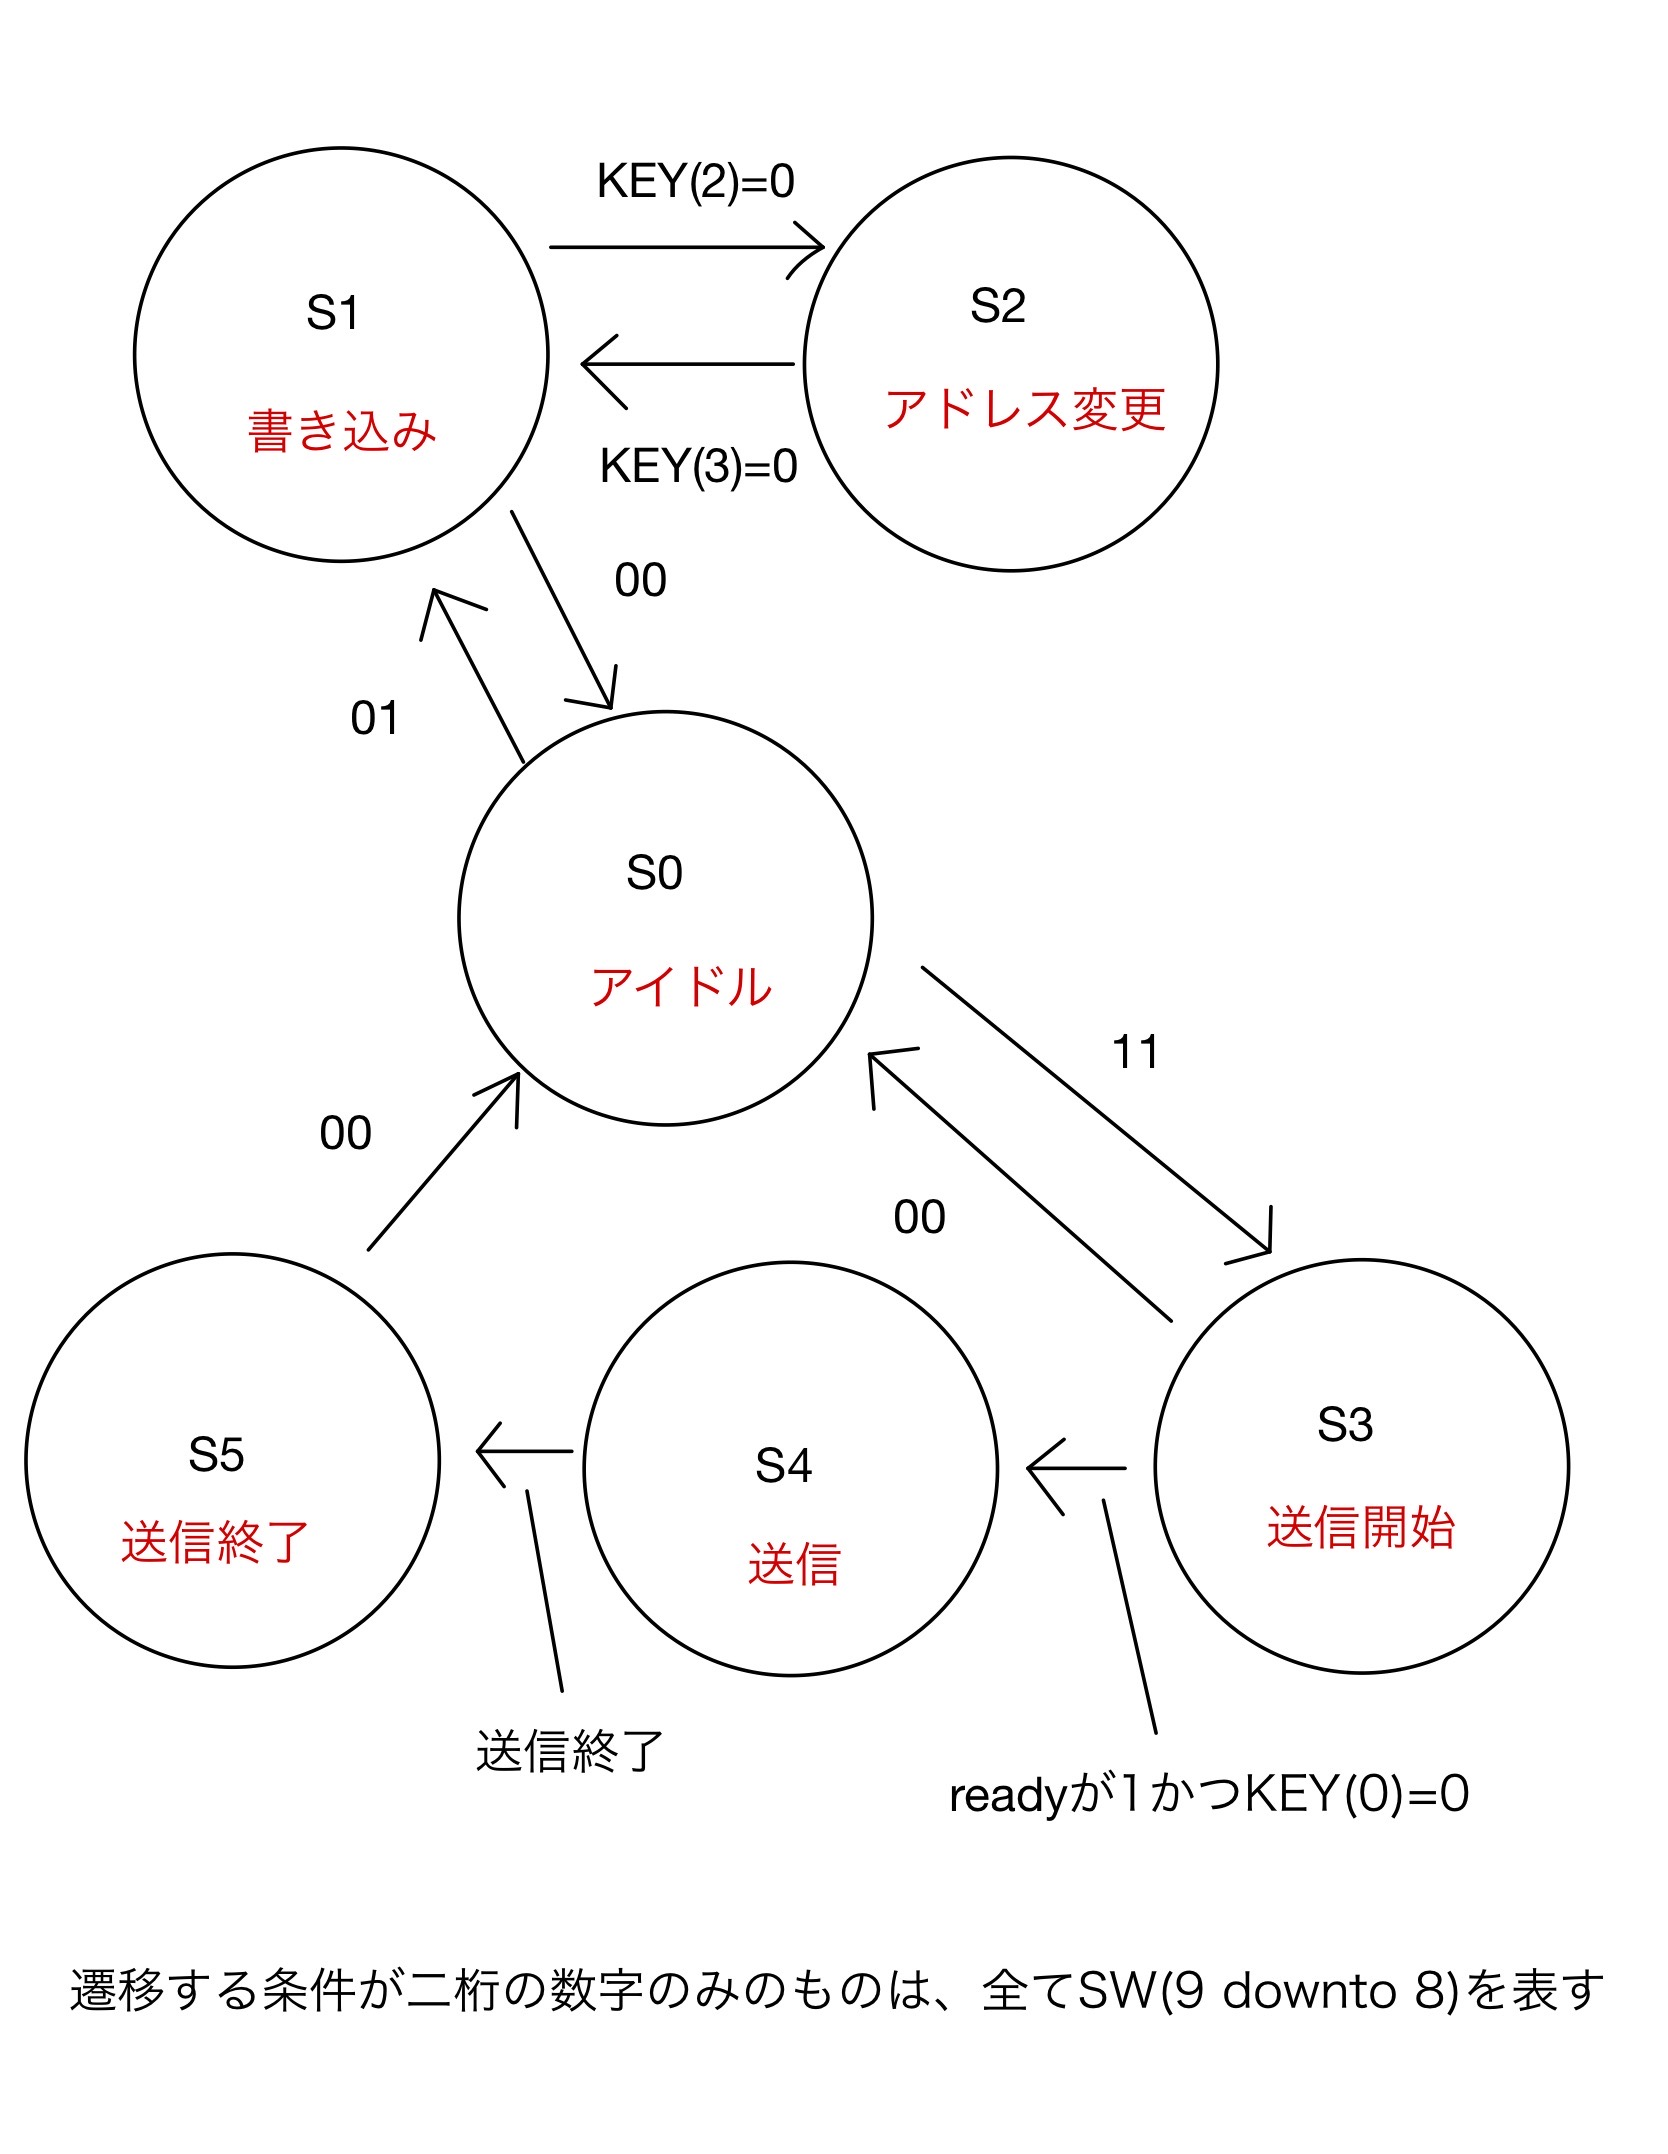
\includegraphics[keepaspectratio, scale=0.1]{state_serve.jpg}
      \caption{送信回路のステート図}
    \end{minipage}
    \begin{minipage}[b]{0.45\linewidth}
      \centering
      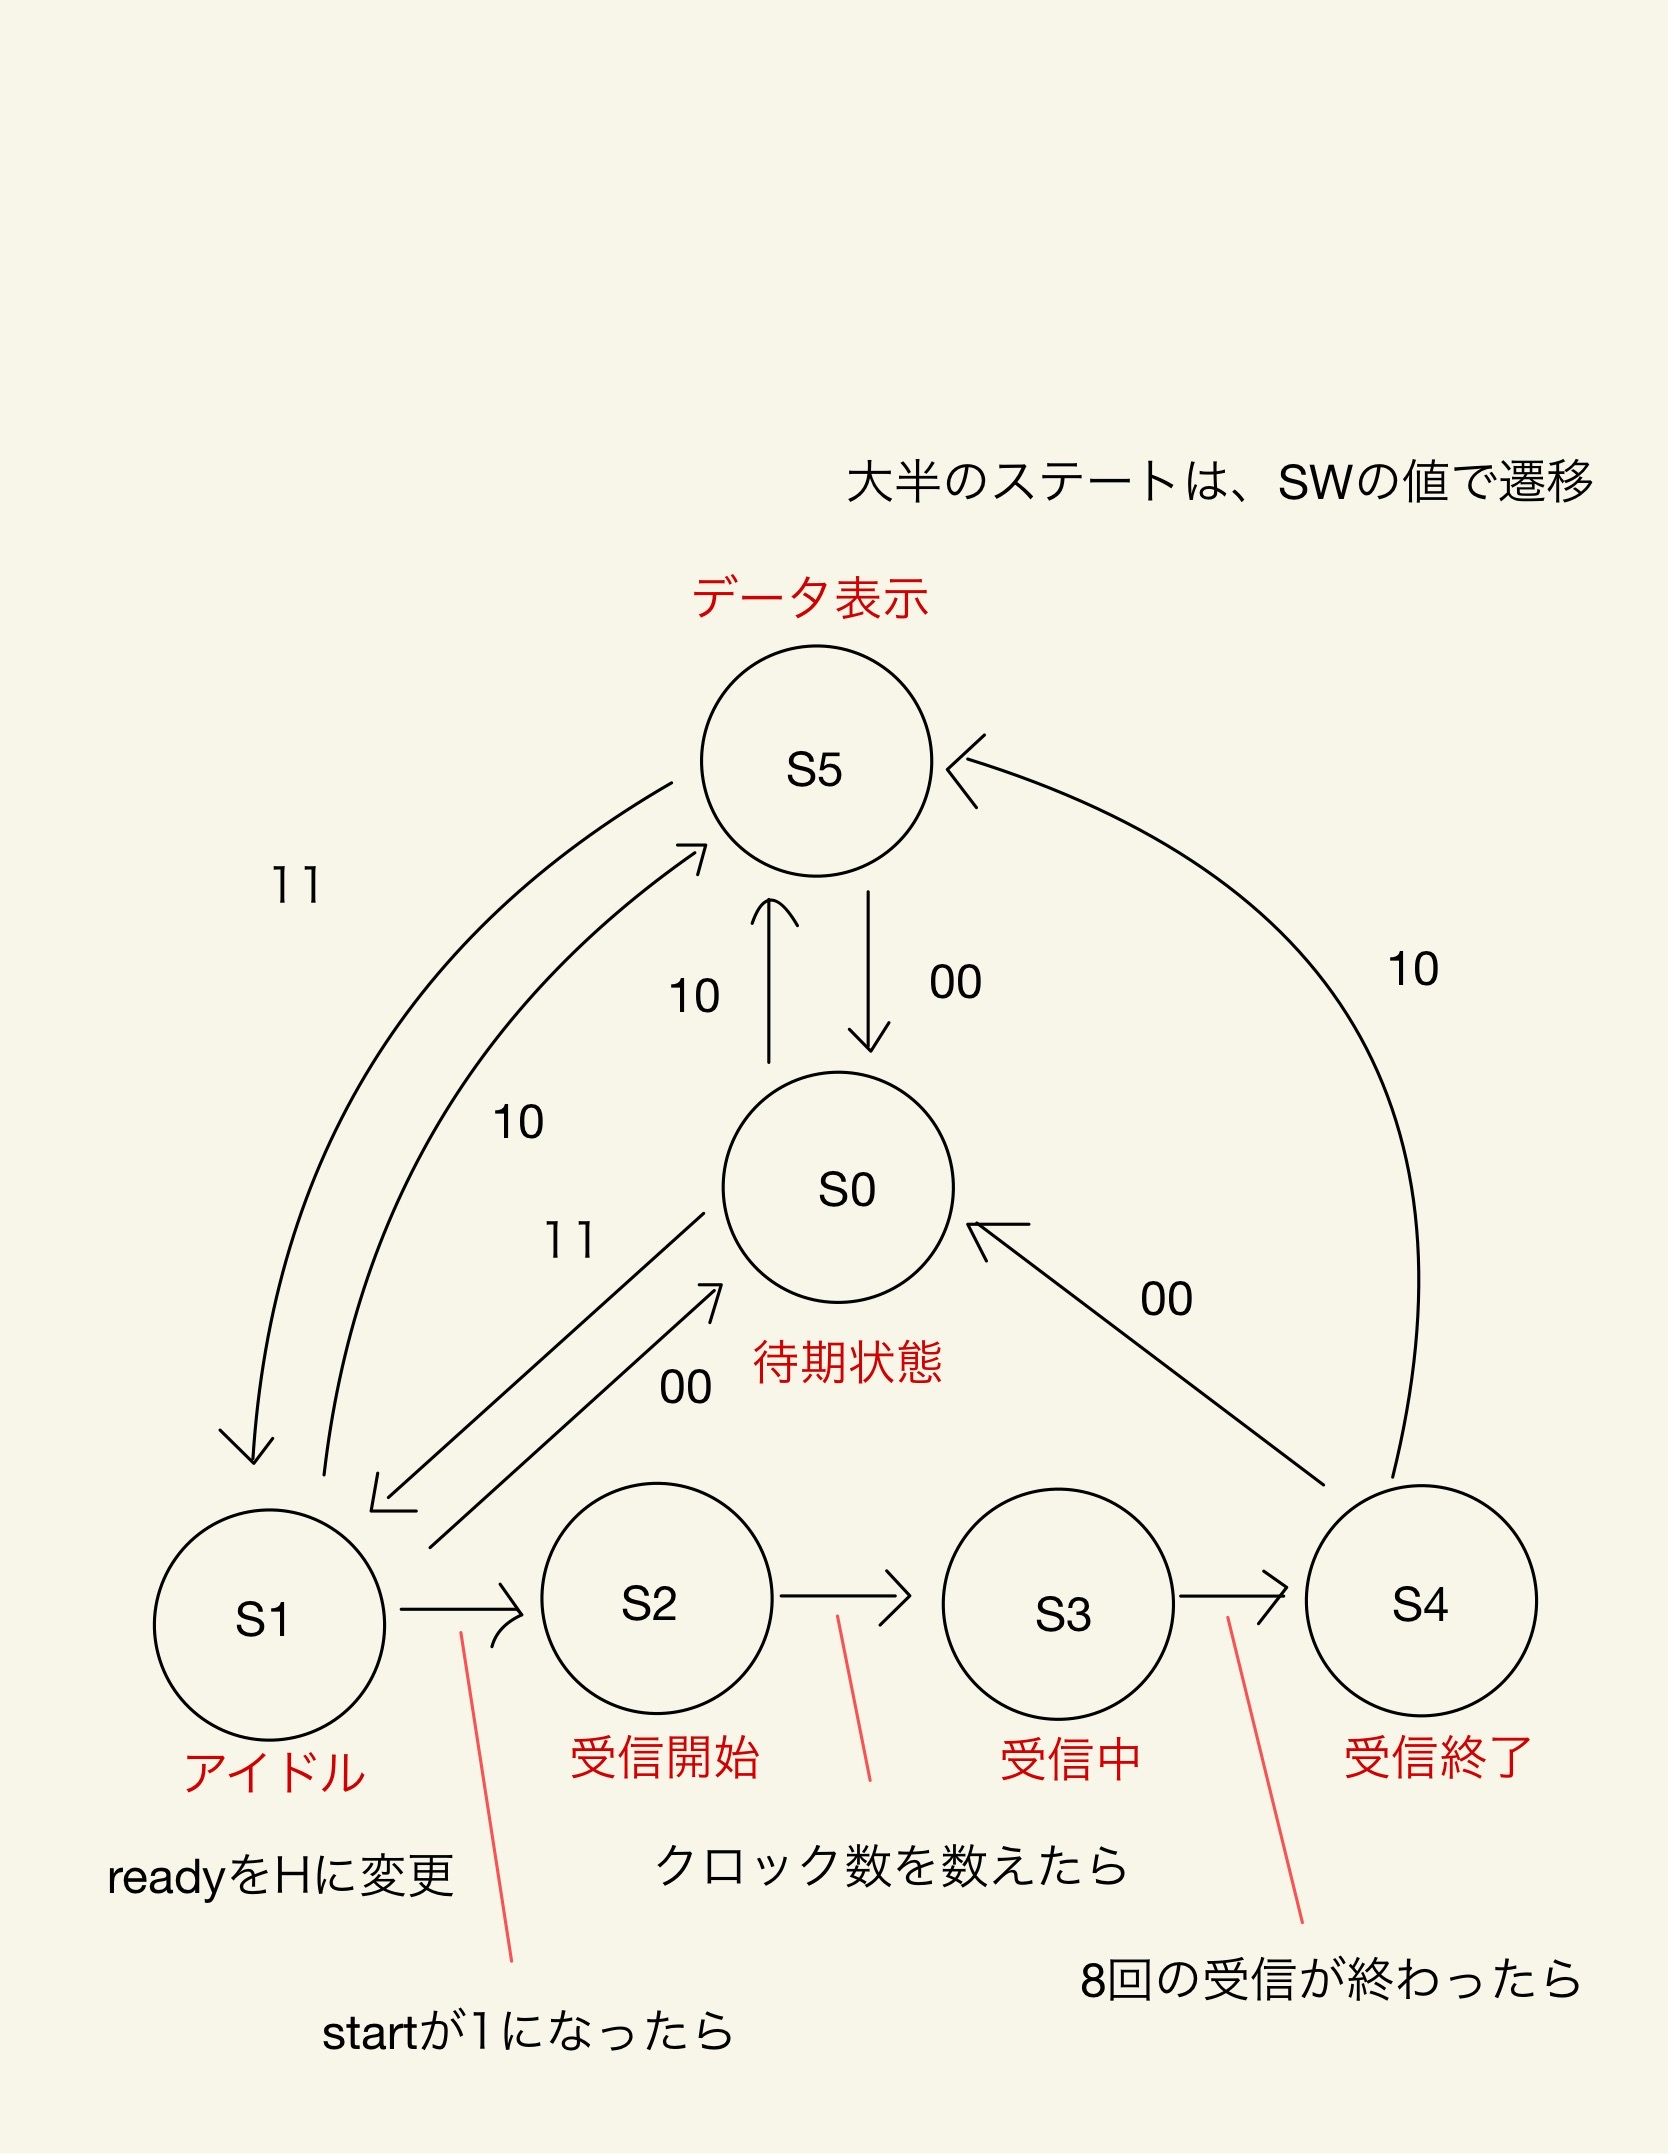
\includegraphics[keepaspectratio, scale=0.1]{state_receive.jpg}
      \caption{受信回路のステート図}
    \end{minipage}
  \end{figure}
\section{送受信回路の設計内容}
\subsection{送信回路の設計}
送信回路の設計にあたって使用した変数の名前とその役割の対応は以下の表2のとおりである.


以下では図1のそれぞれのステートにおける処理を記述する.また,Listing1は3.1の末尾に添付したのは送信回路の
\subsubsection{アイドル状態}
s0であるアイドル状態について記述する.32ビットのベクトルであるSWの8から9ビット目を参照しその値によって次の遷移先を決定する.01ならs1に遷移し,11ならs3に遷移する.
それ以外であればs0にとどまり続ける.また,s1に遷移する際にはwadrを000に,key2\_fragを0に,write\_inを0000に初期化する.
これらの変数の具体的な働きは後述する.また,このときにKEY(0)が0であるかどうかを判定し0であればkey2\_fragを1としているがこれは
テストベンチのKEYの切り替わりをステートの遷移後に計測しているとデータを書き込むのに間に合わなかったので追加した.
\subsubsection{書き込み状態}
s1である書き込み状態について記述する.KEY(0)が0になっている,即ちKEY(0)が押されるとkey2\_fragという変数が1となる.このkey2\_fragという変数はKEY(2)が押されたことを記憶しておく変数である.
そしてこのkey2\_fragが1であればkey2\_frag,KEY(3)が押されたかどうかを判定するkey3\_fragを0にしてwrite\_inに現在のdinの値を格納する.dinはram1の入力であり
一度write\_inに退避させておくことで次のアドレス変更状態にいる際にデータが変更されても書き込むデータ自体はKEY(2)を押したタイミングでのデータであり続けるからである.そしてその後
s2に遷移する.また,s0の時と同様にSWの8から9ビットが00であればs0に遷移し,以上どの分岐にも当てはまらない場合にはs1にとどまり続ける.

\subsubsection{アドレス変更状態}
s2であるアドレス変更状態について記述する.KEY(2)やKEY(3)が押されるとそれぞれのfragの変数が1となる.
key3\_fragが1であるかどうかを判定し,1であればkey3\_fragを0にしwadrを1だけ増やす.これにより加算される前のwadrの
値に対応するデータの値が確定する.そして分岐に当てはまらなければs2にとどまり続ける.
\subsubsection{送信開始状態}
s3である送信開始について記述する.SWの8から9ビットが00であればs0に遷移する.次に受信側が送ってくるreadyが1であるかどうかを判定する.
readyが1でなければs3にとどまり続け以降の判定は行わない.readyが1のときはKEY(0)が0かどうかを判定する.0であればradrを000に,countを1に初期化してs4に遷移する.
\subsubsection{送信状態}
s4である送信状態について記述する.
\subsubsection{送信終了状態}
s5である送信終了状態について記述する.SWの8から9ビットが00であればradr,clk\_tx\_last,count,count\_send,count\_clkを初期化してs0に遷移する.それ以外の時はs5にとどまり続ける.
\begin{lstlisting}[caption=送信回路のコード,label=fuga]
library ieee;
use ieee.std_logic_1164.all;
use ieee.std_logic_unsigned.all;
use IEEE.NUMERIC_STD.all;

entity tx is
  generic(N: integer := 32;
          K: integer := 4;
          W: integer := 3);
  port(
    CLOCK_50, RESET_N: in std_logic;
    -- KEY(0): start button
    -- KEY(2): write enable
    -- KEY(3): address increment
    KEY: in std_logic_vector(3 downto 0);
    -- SW(9 downto 8): mode
    -- SW(3 downto 0): din
    SW: in std_logic_vector(9 downto 0);
    -- GPIO_1(3 downto 0): data bits
    -- GPIO_1(4): start bit
    -- GPIO_1(5): ready bit
    GPIO_1: inout std_logic_vector (35 downto 0);
    -- LEDR: for debug
    LEDR: out std_logic_vector (9 downto 0);
    HEX0, HEX1, HEX2, HEX3, HEX4, HEX5: out std_logic_vector(6 downto 0));
end tx;

architecture rtl of tx is
  constant cnt_max: std_logic_vector(31 downto 0):= X"000003FF";
  type state_type is (s0, s1, s2, s3 , s4 , s5);
  signal state: state_type;
  signal sout: std_logic_vector (3 downto 0);
  signal clk, xrst: std_logic;
  signal enable: std_logic;
  signal clk_tx: std_logic;
  signal start: std_logic;
  signal ready: std_logic;
  signal we: std_logic;
  signal wee: std_logic;
  signal wadr, radr, adr: std_logic_vector (2 downto 0);
  signal din, dout: std_logic_vector (3 downto 0);
  signal debug0, debug1, debug2: std_logic_vector (3 downto 0);
  signal enter_1, enter_3, enter_5: std_logic_vector (3 downto 0);
  signal count_send, count_read, count_write, count_clk, count : integer := 0;
  signal clk_tx_last, finish,key2_frag, key3_frag: std_logic;
  signal write_in, first: std_logic_vector (3 downto 0);
  
  component clock_gen
    generic(N: integer);
    port(clk, xrst: in std_logic;
         enable: in std_logic;
         cnt_max: in std_logic_vector (N-1 downto 0);
         clk_tx: out std_logic);
  end component;
  
  component ram_WxK
    generic(K: integer;
            W: integer);
    port(clk: in std_logic;
         din: in std_logic_vector (K-1 downto 0);
         wadr: in std_logic_vector (W-1 downto 0);
         radr: in std_logic_vector (W-1 downto 0);
         we: in std_logic;
         dout: out std_logic_vector (K-1 downto 0));
  end component;
  
  component seven_seg_decoder is
    port(clk: in std_logic;
         xrst: in std_logic;
         din: in std_logic_vector(3 downto 0);
         dout: out std_logic_vector(6 downto 0));
  end component;
  
begin
  clk <= CLOCK_50;
  xrst <= RESET_N;
  din <= SW(3 downto 0);
  we <= not KEY(2);
  clk_tx_last <= '0';
  ready <= GPIO_1(5);

  cg1: clock_gen generic map(N => N) port map(clk => clk, xrst => xrst, enable => enable, cnt_max => cnt_max, clk_tx => clk_tx);
  ram1: ram_WxK generic map(K => K, W => W) port map(clk => clk, din => write_in, wadr => wadr, radr => radr, we => key3_frag, dout => dout);
  ssd0: seven_seg_decoder port map(clk => CLOCK_50, xrst => RESET_N, din => "0000", dout => HEX0);
  ssd1: seven_seg_decoder port map(clk => CLOCK_50, xrst => RESET_N, din => enter_1, dout => HEX1);
  ssd2: seven_seg_decoder port map(clk => CLOCK_50, xrst => RESET_N, din => "0000", dout => HEX2);
  ssd3: seven_seg_decoder port map(clk => CLOCK_50, xrst => RESET_N, din => enter_3, dout => HEX3);
  ssd4: seven_seg_decoder port map(clk => CLOCK_50, xrst => RESET_N, din => "0000", dout => HEX4);
  ssd5: seven_seg_decoder port map(clk => CLOCK_50, xrst => RESET_N, din => enter_5, dout => HEX5);

process(xrst,clk)
begin
  if(xrst = '0')then
    state <= s0;
    enable <= '0';
    wadr <= "000";
    radr <= "000";
    finish <= '0';
    start <= '0';
		
  elsif(clk'event and clk = '1')then 
    case state is
      when s0 =>
        enable <= '0';
	    finish <= '0';
		
        if(sw(9 downto 8) = "01")then 
            wadr <= "000";
            key2_frag <= '0';
            write_in <= "0000";
            if(KEY(2) = '0')then
                key2_frag <= '1';
                end if;
            state <= s1;                  
        elsif(sw(9 downto 8) = "11")then
            state <= s3;                
        else 
            state <= s0;                 
        end if;


      when s1 =>
        if(KEY(2) = '0')then
            key2_frag <= '1';
        end if;
        if(key2_frag = '1')then
            key3_frag <= '0';
            key2_frag <= '0';
            write_in <= din;
          if(KEY(3) = '0')then
            key3_frag <= '1';
          end if;
	        state <= s2;			
	    elsif(sw(9 downto 8) = "00")then  
          state <= s0;				
	    else
	        state <= s1;		
	    end if;

      when s2 =>
        if(KEY(3) = '0')then
            key3_frag <= '1';
        end if;
        if(KEY(2) = '0')then
            key2_frag <= '1';
        end if;
        if(key3_frag = '1')then
            key3_frag <= '0';
            wadr <= wadr + 1;
            state <= s1;
        else
            state <= s2;
        end if;
				
      when s3 =>
	    if(sw(9 downto 8) = "00")then
	        state <= s0;				
	    elsif(ready = '1')then
            if(KEY(0) = '0')then 
                GPIO_1(4) <= '1';
                radr <= "000";
                count <= 1;
                state <= s4;                        
            end if;
        else 
	      state <= s3;
		end if;			
       

      when s4 =>
        if(finish = '0')then 
        enable <= '1';
        if(clk_tx = '1')then
            if(clk_tx_last = '0')then	
                clk_tx_last <= '1';
                start <= '0';
                finish <= '1';
                enable <= '0';
            end if;
        else 
            start <= '1';
            clk_tx_last <= '0';
            count_clk <= count_clk + 1;
        end if;
        elsif(count_send = 8)then
            count_send <= 0;
            state <= s5;
        else
            count <= count + 1;
            if(count = count_clk -1)then
                radr <= radr + 1;
                enter_1 <= dout;
                enter_3 <= "0" & radr;
                enter_5 <= "000" & GPIO_1(4);
                count_send <= count_send + 1;
                count <= 0;
            end if;
            state <= s4;
        end if;	

    when s5 =>
        if(SW(9 downto 8) = "00")then
            adr <= "000";
            clk_tx_last <= '0';
            count <= 0;
            count_send <= 0;
            count_clk <= 0;
            state <= s0;
        else  
            state <= s5;
        end if;
      end case;
    end if;
GPIO_1(4) <= start;
GPIO_1(0) <= enter_1(0);
GPIO_1(1) <= enter_1(1);
GPIO_1(2) <= enter_1(2);
GPIO_1(3) <= enter_1(3);
end process;
end rtl;



\end{lstlisting}

\subsection{受信回路の設計}
\section{テストベンチによる動作確認内容・結果}
\subsection{送信回路の動作結果}
\subsection{受信回路の動作結果}
\section{非同期通信回路作成における注意点などの考察}
\section{教員・TAによる動作確認時刻}
1月23日時分
\end{document}